\clearpage
%%%%%%%%%%%%%%%%%%%%%%%%%%%%%%%%%%%%%%%%%%%%%%%%%%%%%%%%%%%%%%%%%%%%%%%%%%%%%%%%%
%%        %%%        %%%        %%%        %%%        %%%         %%%  %%%%  %%%
%%  %%%%%%%%%  %%%%%%%%%  %%%%%%%%%%%%  %%%%%%%%%  %%%%%%  %%%%%  %%%    %%  %%%
%%        %%%        %%%  %%%%%%%%%%%%  %%%%%%%%%  %%%%%%  %%%%%  %%%  %  %  %%%
%%%%%%%%  %%%  %%%%%%%%%  %%%%%%%%%%%%  %%%%%%%%%  %%%%%%  %%%%%  %%%  %%    %%%
%%        %%%        %%%        %%%%%%  %%%%%%        %%%         %%%  %%%   %%%
%%%%%%%%%%%%%%%%%%%%%%%%%%%%%%%%%%%%%%%%%%%%%%%%%%%%%%%%%%%%%%%%%%%%%%%%%%%%%%%%%
 \section{ヒストグラムを描く}

 \begin{itembox}{\texttt{hist1.cpp}}
\begin{verbatim}
	#include "TH1.h"
	#include <iostream>

	TH1D *hist1(){
	  std::cout << "Start!!" << std::endl;
	  TH1D *h = new TH1D("h","h",100,-5.,5.);
	  h->FillRandom("gaus") ;
	  h->Draw();
	  return h;
	}
\end{verbatim}
 \end{itembox}

 まずは実行してみてほしい。
 すると、
 \begin{figure}[htbp]
  \begin{center}
   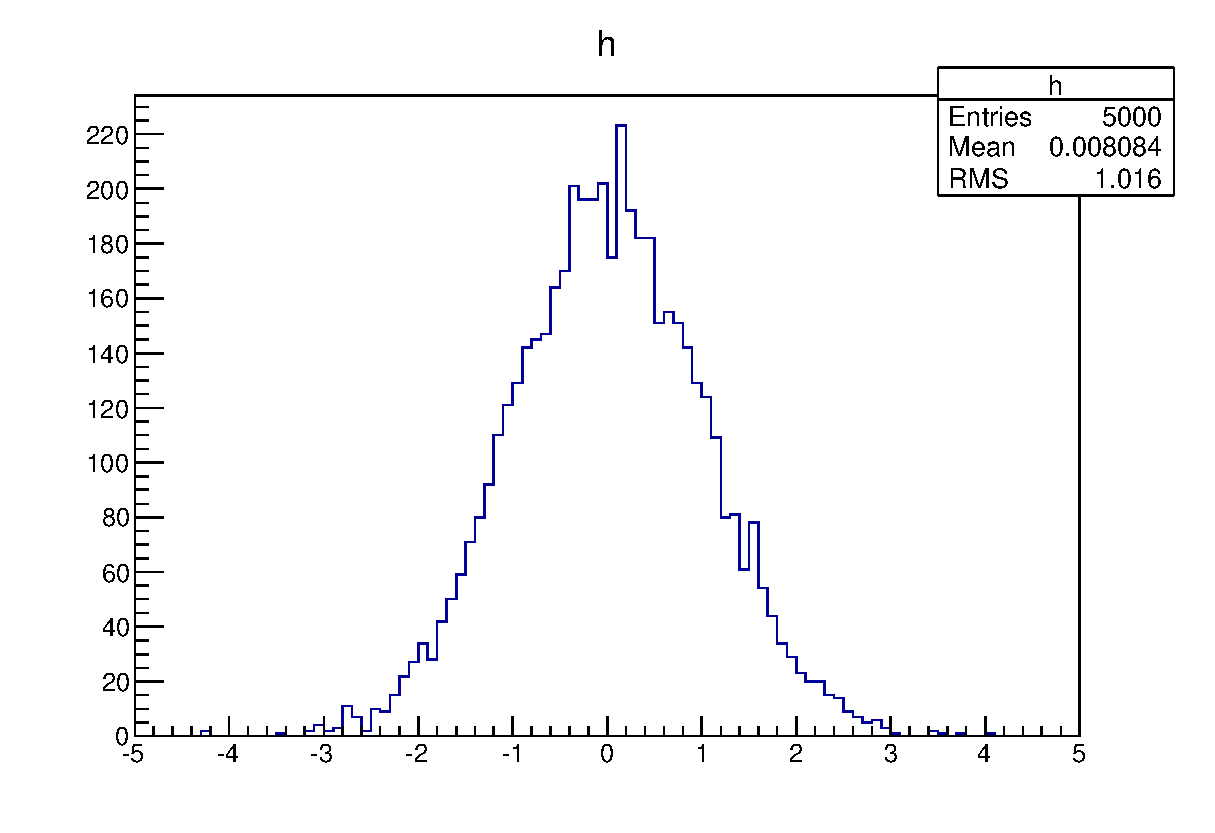
\includegraphics[width = 100mm]{./picture/hist1canvas1.eps}
  \end{center}
  \caption{ヒストグラムの図}
  \label{Fig:hist1canvas1}
 \end{figure}

  \subsection{練習}

  \begin{enumerate}
   \item ヒストグラムを統計誤差付きで評価せよ
	 \begin{description}
	  \item[ヒント] \url{http://root.cern.ch/root/html/TH1.html#TH1:Draw}
	  \item[ヒント] \url{http://root.cern.ch/root/html/THistPainter.html#HP01a}
	  \item[ヒント] \url{http://root.cern.ch/root/html/THistPainter.html#HP01b}
	 \end{description}
   \item ヒストグラムの最大値を取得せよ。
	 \begin{description}
	  \item[ヒント] \url{http://root.cern.ch/root/html/TH1.html#TH1:GetMaximum}
	 \end{description}
   \item ヒストグラムの最大値が納められたbinのbin番号を取得せよ。
	 \begin{description}
	  \item[ヒント] \url{http://root.cern.ch/root/html/TH1.html#TH1:GetMaximumBin}
	 \end{description}
   \item ヒストグラムの最大値が納められたbinのエラーの値を取得せよ。
	 \begin{description}
	  \item[ヒント] \url{http://root.cern.ch/root/html/TH1.html#TH1:GetBinError}
	 \end{description}
   \item GUIを用いてグリッドを描け。最終的に図\ref{Fig:hist1canvas2}のように描け。
	 \begin{description}
	  \item[ヒント] GUIでは<View>から<Editor>を選択する。
		     するとキャンバスの左側に様々な編集ツールが表示される。
		     \begin{figure}[htbp]
		      \begin{center}
		       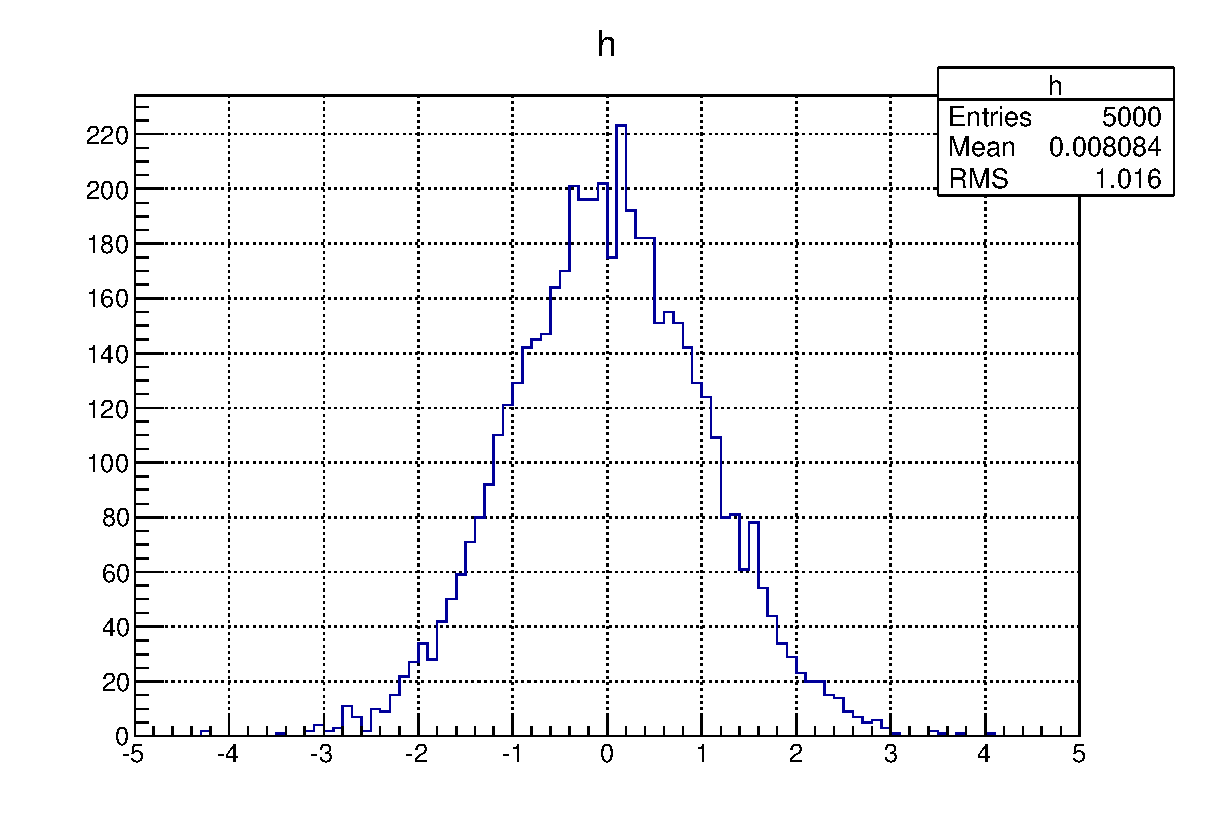
\includegraphics[width = 100mm]{./picture/hist1canvas2.eps}
		      \end{center}
		      \caption{グリッドを描いたヒストグラム}
		      \label{Fig:hist1canvas2}
		     \end{figure}
	 \end{description}
   \item \ROOT で\verb|h->Draw();|を行ったとき、 \\
	 \verb|Info in <TCanvas::MakeDefCanvas>: created default TCanvas with name c1| \\
	 というメッセージが出ただろう。文字どおり、c1というキャンバスが作られ、そこにhが描画されている。
	 c1を"c1.eps"として保存せよ。
	 \begin{description}
	  \item[ヒント] \ROOT のキャンバスなどは全て\verb|TObject|からの派生である。\\
		     \url{http://root.cern.ch/root/html/TObject.html#TObject:SaveAs}
	 \end{description}

  \end{enumerate}

  \subsection{解答例}
  \begin{enumerate}
   \item ヒストグラムを統計誤差付きで評価せよ
	 \begin{itembox}{\texttt{hist1sol1.cpp}}
\begin{verbatim}
	...
	TH1D *hist1sol1(){
	  ...
	  h->Draw("E");
	  ...
	}
\end{verbatim}
	 \end{itembox}

   \item ヒストグラムの最大値を取得せよ。
\begin{verbatim}
	root [0] .L hist1.cpp+
	root [1] hist1()
	Start!!
	Info in <TCanvas::MakeDefCanvas>:  created default TCanvas with name c1
	(class TH1D*)0x7f97b4b7bda0
	root [2] h->GetMaximum()
	(const Double_t)2.23000000000000000e+02
\end{verbatim}
   \item ヒストグラムの最大値が納められたbinのbin番号を取得せよ。
\begin{verbatim}
	root [3] h->GetMaximumBin()
	(const Int_t)52
\end{verbatim}
   \item ヒストグラムの最大値が納められたbinのエラーの値を取得せよ。
\begin{verbatim}
	root [4] int maxbinnum = h->GetMaximumBin()
	root [5] h->GetBinError(maxbinnum)
	(const Double_t)1.49331845230680784e+01
\end{verbatim}
   \item GUIを用いてグリッドを描け。最終的に図\ref{Fig:hist1canvas2}のように描け。

   \item c1を"c1.eps"として保存せよ。
\begin{verbatim}
	root [6] c1->SaveAs("c1.eps")
	Info in <TCanvas::Print>: eps file c1.eps has been created
\end{verbatim}
  \end{enumerate}
  